%% -*- TeX-engine: xetex -*-

\documentclass{beamer}

\setbeamertemplate{navigation symbols}{}
\setbeamertemplate{headline}{}
\setbeamertemplate{footline}{}
\setbeamertemplate{itemize items}[triangle]

\defbeamertemplate*{footline}{infolines theme frame plus slide}{
{\hfill
  \insertframenumber / \inserttotalframenumber\hspace*{2ex}
  \vskip0pt%
}}
\setbeamertemplate{footline}[infolines theme frame plus slide]
\setbeamertemplate{frametitle continuation}{}

\usepackage{color}
\definecolor{mauve}{rgb}{0.58,0,0.82}
\definecolor{maroon}{rgb}{0.5,0,0}
\definecolor{dgreen}{rgb}{0,0.5,0}

\usepackage{amsmath}

\usepackage{listings}

\lstdefinelanguage{ocamlgrammar}{
  keywords={match,with,perform,effect,continue,raise},
  otherkeywords={},
  sensitive=true,
  keywordstyle=\color{blue}, % OCaml keywords
  identifierstyle=\color{maroon}\rmfamily\textit,  % nonterminals
  literate={DEF}{::=\;\;}1 {ETC}{$\ldots$}1 {BAR}{\big|}1
                {STAR}{$^*$}1 {LSTAR}{\big(}1 {RSTAR}{\big)$^*$}1
                {OPT}{$^?$}1 {LOPT}{\big(}1 {ROPT}{\big)$^?$}1
                {ROW}{$\Ident{\Row}$}1 {EFF}{$\Ident{\Eff}$}1
}

\lstdefinestyle{ocamlgrammar}
{
  language=ocamlgrammar,
  basicstyle=\ttfamily,
  columns=flexible,
  mathescape=true,
}

\lstdefinestyle{ocaml}
{
  language=[Objective]Caml,
  escapeinside={(**}{*)},
  morekeywords={perform, effect, continue, raise},
  otherkeywords={},
  basicstyle=\ttfamily,
  commentstyle=\color{green},
  keywordstyle=\color{blue},
  stringstyle=\color{mauve},
}

\usepackage{graphicx}

\usepackage{bussproofs}

\newcommand{\Text}[1]{\texttt{#1}}
\newcommand{\Keyword}[1]{{\color{blue}{\Text{#1}}}}
\newcommand{\Var}[1]{#1}
\newcommand{\Op}[1]{{\color{purple}{#1}}}
\newcommand{\Ident}[1]{{\color{maroon}{#1}}}

\newcommand{\Context}{\Var{\Gamma}}
\newcommand{\Et}{\mathrel{\Op{;}}}
\newcommand{\VDash}{\mathrel{\Op{\vdash}}}
\newcommand{\HasType}{\mathrel{\Op{:}}}
\newcommand{\HasEffect}{\mathrel{\Op{!}}}
\newcommand{\Subtype}[2]{{#1}
                         \mathrel{\Op{<:}}
                         {#2}}
\newcommand{\Equal}[2]{{#1}\mathrel{\Op{\cong}}{#2}}

\newcommand{\Or}{\mathbin{|}}
\newcommand{\Row}{\ensuremath{\Delta}}
\newcommand{\Eff}{\ensuremath{\mathcal{E}}}
\newcommand{\Rvar}{\ensuremath{\rho}}
\newcommand{\RowTo}{\xrightarrow{\Row}}

\title{Effective programming}
\subtitle{Bringing algebraic effects and handlers to OCaml}
\author{Leo White\inst{1} \and Stephen Dolan\inst{2} \and Matija Pretnar\inst{3} \and KC
Sivaramakrishnan\inst{2}}
\date{}

\institute{
  \inst{1}%
  Jane Street
  \and
  \inst{2}%
  University of Cambridge
  \inst{3}%
  University of Ljublijana
}

\begin{document}

\frame{\titlepage}

\begin{frame}[c]
\begin{center}
\Huge Algebraic effects and handlers
\end{center}
\end{frame}

\begin{frame}
\frametitle{Algebraic effects and handlers}
\begin{itemize}
\setlength\itemsep{2em}
\item<1-> Algebraic effecects originally introduced to study the semantics
  of computational effects.
\begin{itemize}
\item[--] \emph{Algebraic Operations and Generic Effects} \\ Plotkin and Power, 2002
\end{itemize}
\item<2-> The addition of handlers turned them into a construct for
  implementing such effects.
\begin{itemize}
\item[--] \emph{Handlers of Algebraic Effects} \\ Plotkin and Pretnar, 2009
\end{itemize}
\end{itemize}
\end{frame}

\begin{frame}[fragile]
\frametitle{Simple example}
\begin{lstlisting}[style=ocaml]
let f () =
  (perform Get) + (perform Get) + 2

match f () with
| ret -> ret
| effect Get, k -> continue k 9

(** {\color{dgreen}-: int = 20} *)

match f () with
| ret -> ret
| effect Get, k -> continue k 99

(** {\color{dgreen}-: int = 200} *)
\end{lstlisting}
\end{frame}

\begin{frame}[fragile]
\frametitle{Syntax}
\begin{block}{Performing effects}
\begin{lstlisting}[style=ocamlgrammar]
e DEF ETC     BAR perform E eOPT
\end{lstlisting}
\end{block}
\begin{block}{Handling effects}
\begin{lstlisting}[style=ocamlgrammar]
e DEF ETC
   BAR   match e with
     LSTAR | x -> e RSTAR
     LSTAR | effect E xOPT, x -> e RSTAR
\end{lstlisting}
\end{block}
\begin{block}{Resuming a continuation}
\begin{lstlisting}[style=ocamlgrammar]
e DEF ETC     BAR continue e e
\end{lstlisting}
\end{block}
\end{frame}

\begin{frame}[fragile]
\frametitle{Typing (unchecked)}
\begin{prooftree}
\AxiomC{$\Var{E} \HasType \Var{A} \to \Var{B}$}
\AxiomC{$\Context \VDash \Var{e} \HasType \Var{A}$}
\alwaysSingleLine
\BinaryInfC{$\Context \VDash \Keyword{perform}
             \; \Var{E} \; \Var{e} \HasType \Var{B}$}
\end{prooftree}
\begin{prooftree}
\AxiomC{$\Context \VDash \Var{e} \HasType
        \Text{(} \Var{A} \Text{,} \Var{B} \Text{)} \, \Text{cont}$}
\AxiomC{$\Context \VDash \Var{e^\prime} \HasType \Var{A}$}
\alwaysSingleLine
\BinaryInfC{$\Context \VDash
            \Keyword{continue}\;\Var{e}\;\Var{e^\prime} \HasType \Var{B}$}
\end{prooftree}
\end{frame}

\begin{frame}[fragile]
\frametitle{Typing (unchecked)}
\begin{prooftree}
\alwaysNoLine
\AxiomC{$\Context \VDash \Var{e} \HasType \Var{A}$}
\UnaryInfC{$\Context \Et \Var{x} \HasType \Var{A} \VDash
            \Var{e^\prime} \HasType \Var{B}$}
\AxiomC{$E_i \HasType \Var{C_i} \to \Var{D_i}$}
\UnaryInfC{$\Context \Et \Var{x_i} \HasType \Var{C_i} \Et \Var{k_i} \HasType
            \Text{(} \Var{D_i} \Text{,} \Var{B} \Text{)} \,\Text{cont} \VDash
            \Var{e^{\prime\prime}_i} \HasType \Var{B}$}
\alwaysSingleLine
\BinaryInfC{$\Context \VDash
            \begin{aligned}
           & \Keyword{match} \; \Var{e} \; \Keyword{with} \\
           & \Text{|} \; \Var{x} \; \Text{->} \; \Var{e^\prime} \\
           & \Text{|} \; \Keyword{effect} \; E_i \; \Var{x_i} \Text{,}
               \; \Var{k_i} \; \Text{->} \; \Var{e^{\prime\prime}_i}
            \end{aligned}
            \HasType \Var{B}$}
\end{prooftree}
\end{frame}


\begin{frame}[fragile]
\frametitle{Semantics}
\lstinline[style=ocamlgrammar]{v DEF ETC} (values)\\
\lstinline[style=ocamlgrammar]{r DEF v BAR   effect E v v} (results)\\
\lstinline[style=ocamlgrammar]{$\mathcal{C}$[_] DEF ETC} (delimited contexts)
\\[2em]
\begin{equation*}
\mathcal{C}[\Keyword{perform}\;E\;v] \longrightarrow
            \Keyword{effect}\;E\;v\;(\lambda x . \mathcal{C}[x])
\end{equation*}
\begin{equation*}
\Keyword{continue}\;v\;v^\prime \longrightarrow v\;v^\prime
\end{equation*}
\end{frame}

\begin{frame}[fragile]
\frametitle{Semantics}
\begin{equation*}
\begin{aligned}
 & \Keyword{match} \; v \; \mathtt{with} \\
 & | \; x \; \Text{->} \; e \\
 & | \; \Keyword{effect} \; E_i \; x_i\Text{,} \; k_i \;
     \Text{->} \; e^\prime_i
\end{aligned}
\longrightarrow
e[v/x]
\end{equation*}
\end{frame}


\begin{frame}[fragile]
\frametitle{Semantics}
\begin{equation*}
\begin{aligned}
 & \Keyword{match} \; \Keyword{effect}\;E\;v\;v^\prime \; \Keyword{with} \\
 & \Text{|} \; x \; \Text{->} \; e \\
 & \Text{|} \; \Keyword{effect} \; E_i \; x_i \Text{,} \; k_i \;
     \Text{->} \; e^\prime_i
\end{aligned}
\longrightarrow
e^\prime_j[v/x_j, v_{cont}/k_j]
\end{equation*}
\\[2em]
where $E = E_j$ and
\begin{equation*}
v_{cont} = \lambda y.
\begin{aligned}
 & \Keyword{match} \; v^\prime y \; \Keyword{with} \\
 & \Text{|} \; x \; \Text{->} \; e \\
 & \Text{|} \; \Keyword{effect} \; E_i \; x_i \Text{,} \; k_i \;
     \Text{->} \; e^\prime_i
\end{aligned}
\end{equation*}
\end{frame}

\begin{frame}[fragile]
\frametitle{Semantics}
\begin{multline*}
\mathcal{C} \Bigg[ \;
\begin{aligned}
 & \Keyword{match} \; \Keyword{effect}\;E\;v\;v^\prime \; \Keyword{with} \\
 & \Text{|} \; x \; \Text{->} \; e^\prime \\
 & \Text{|} \; \Keyword{effect} \; E_i \; x_i\Text{,} \; k_i \;
     \Text{->} \; e^{\prime\prime}_i
\end{aligned}
\; \Bigg] \\
\longrightarrow \\
\Keyword{effect} \; E \; v \;
(\lambda y.
\mathcal{C} \Bigg[ \;
\begin{aligned}
 & \Keyword{match} \; v^\prime \; y \; \Keyword{with} \\
 & | \; x \; \Text{->} \; e^\prime \\
 & | \; \Keyword{effect} \; E_i \; x_i\Text{,} \; k_i \;
     \Text{->} \; e^{\prime\prime}_i
\end{aligned}
\; \Bigg] )
\end{multline*}
\\[2em]
where $\forall j. E \neq E_j$
\end{frame}


\begin{frame}[fragile]
\frametitle{Examples: Exceptions}
\begin{lstlisting}[style=ocaml]
let raise (msg : string) : 'a =
  perform Raise msg

let run f =
  match f () with
  | ret -> Ok ret
  | effect Raise msg, k -> Error msg
\end{lstlisting}
\end{frame}

\begin{frame}[fragile]
\frametitle{Examples: State}
\begin{lstlisting}[style=ocaml]
let put (v : int) : unit = perform Put v

let get () : int = perform Get

let run init f =
  let comp =
    match f () with
    | ret ->
        (fun s -> ret)
    | effect Put s', k ->
        (fun s -> continue k () s')
    | effect Get, k ->
        (fun s -> continue k s s)
  in
  comp init
\end{lstlisting}
\end{frame}

\begin{frame}[fragile]
\frametitle{Examples: Choice}
\begin{lstlisting}[style=ocaml]
let select () : bool = perform Select

let run_true f =
  match f () with
  | ret -> ret
  | effect Select, k ->
      continue k true

let run_all f =
  match f () with
  | ret -> [ret]
  | effect Select, k ->
      continue k true @ continue k false
\end{lstlisting}
\end{frame}

% Could also add a comparison with delimited continuations

\begin{frame}[c]
\begin{center}
\Huge Algebraic effects in OCaml
\end{center}
\end{frame}

\begin{frame}[fragile]
\frametitle{Defining (unchecked) effects}
\begin{lstlisting}[style=ocaml]
effect Get : int

effect Put : int -> unit
\end{lstlisting}
\end{frame}

\begin{frame}[fragile]
\frametitle{Default handlers}
\begin{lstlisting}[style=ocaml]
effect Yield : unit
  with function Yield -> ()
\end{lstlisting}
\end{frame}

\begin{frame}[fragile]
\frametitle{Affine continuations}
\begin{lstlisting}[style=ocaml]
let select () : bool = perform Select

let run_all f =
  match f () with
  | ret -> [ret]
  | effect Select, k ->
      continue k true @ continue k false

let _ = run_all select
(**{\color{red}Exception: Invalid\_argument "continuation already taken"}*)
\end{lstlisting}
\end{frame}

\begin{frame}
\frametitle{Implementation}
\begin{itemize}
\setlength\itemsep{2em}
\item Fibers: Heap allocated, dynamically resized stacks
\begin{itemize}
\item[--] ~10s of bytes
\end{itemize}
\item Entering an effect handler creates a fresh fiber
\item Call stack becomes a linked list of fibers
\end{itemize}
\end{frame}

\begin{frame}[fragile]
\frametitle{Implementation}
\begin{center}
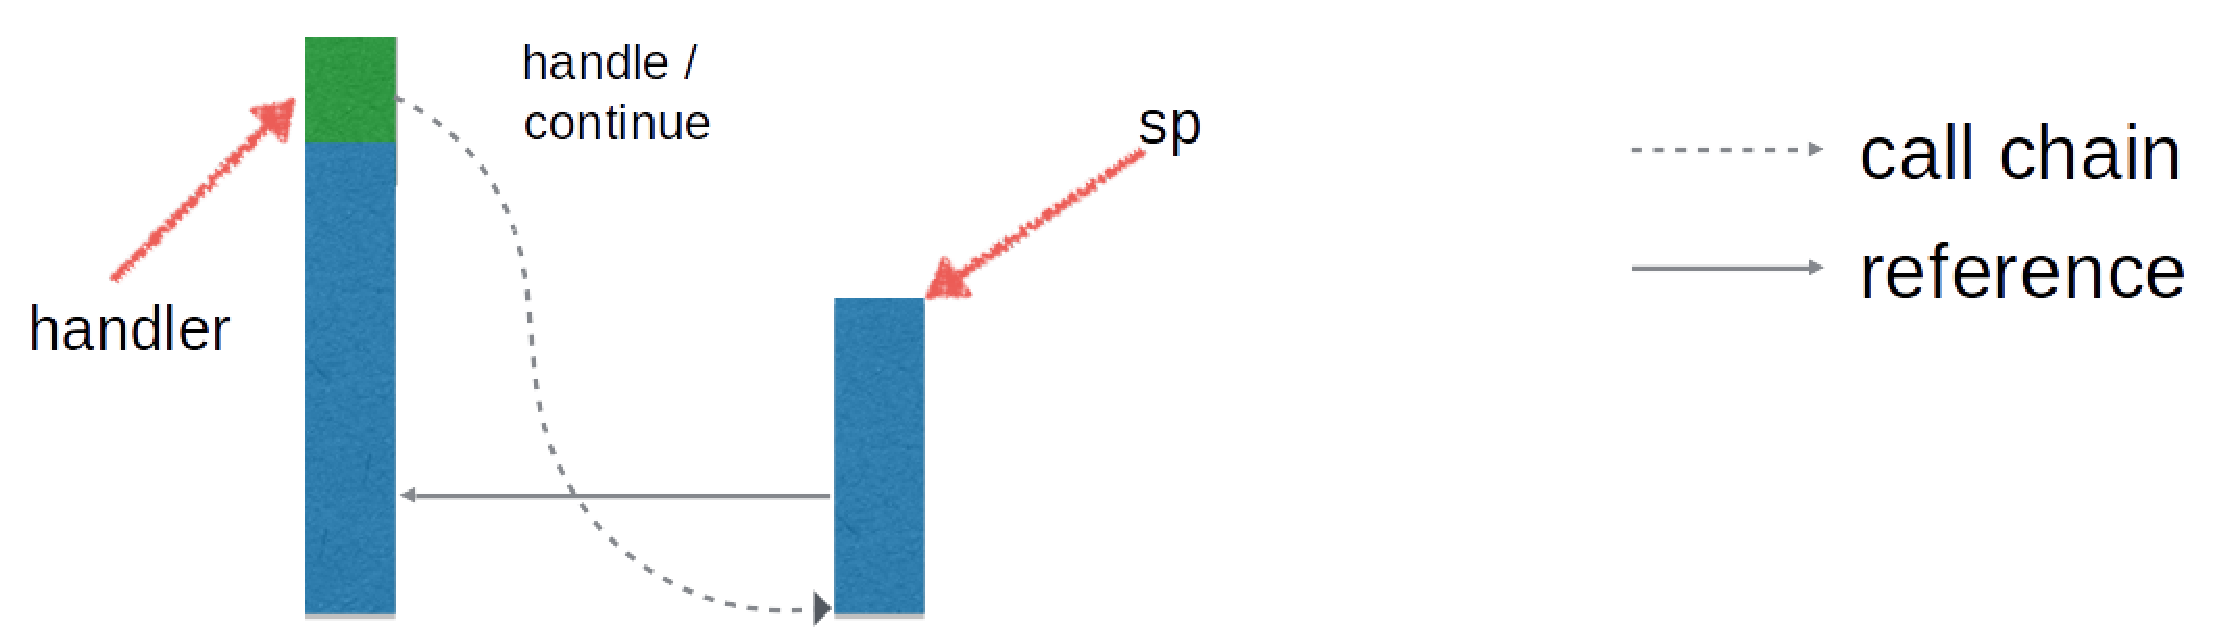
\includegraphics[width = 0.9\textwidth]{./imp1}
\end{center}
\end{frame}

\begin{frame}[fragile]
\frametitle{Implementation}
\begin{center}
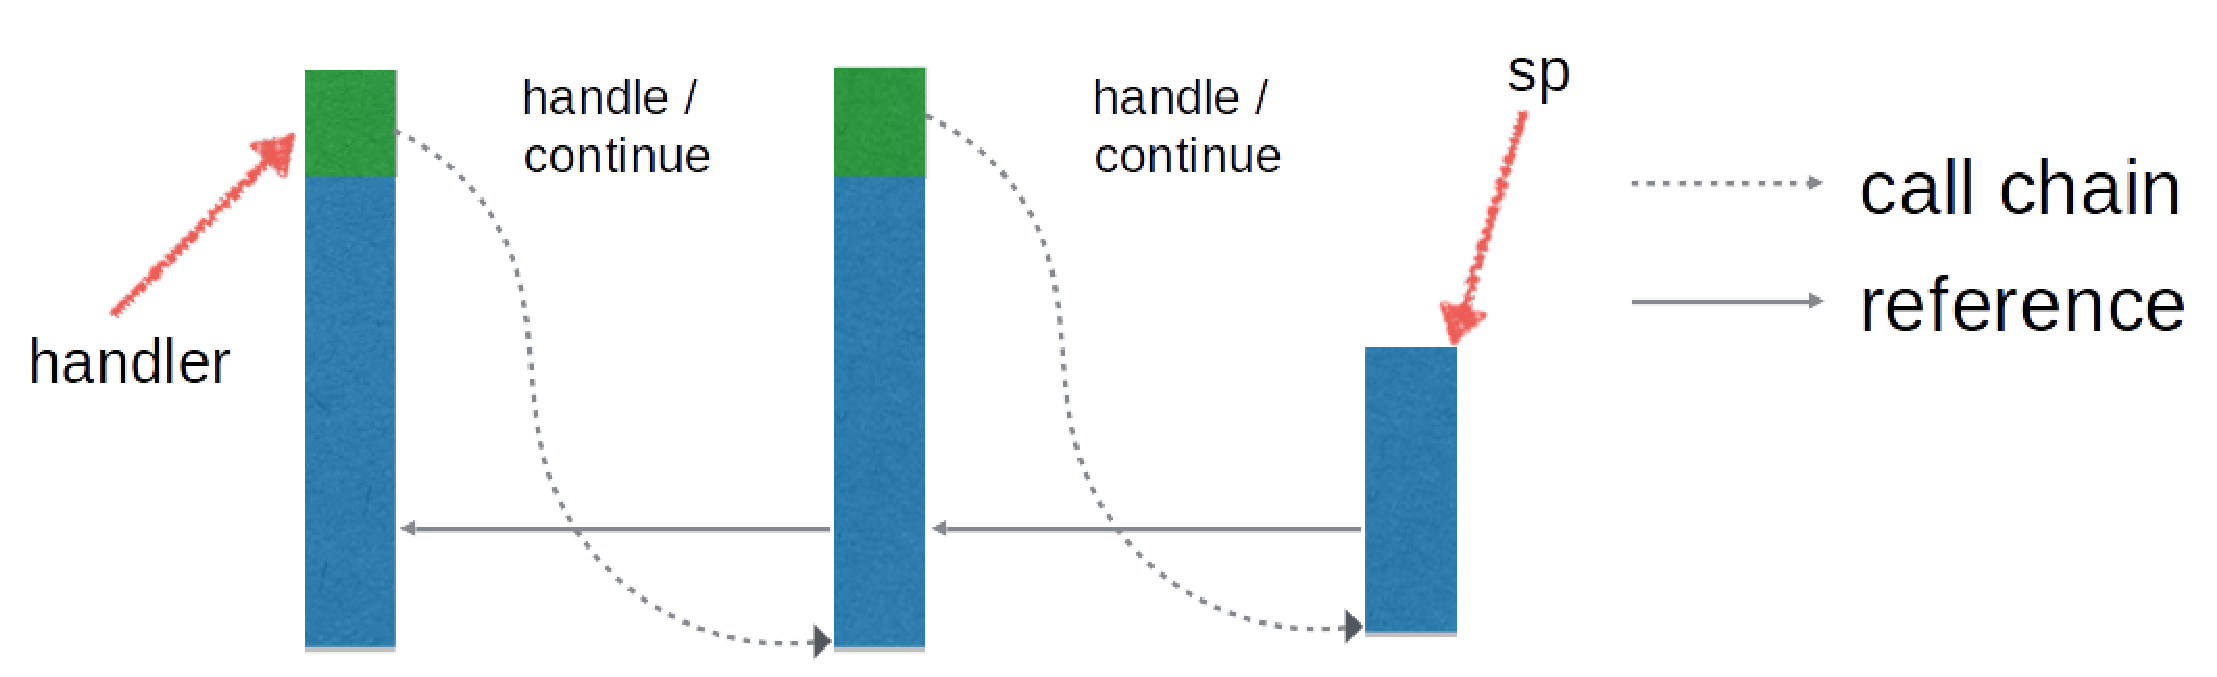
\includegraphics[width = 0.9\textwidth]{./imp2}
\end{center}
\end{frame}

\begin{frame}[fragile]
\frametitle{Implementation}
\begin{center}
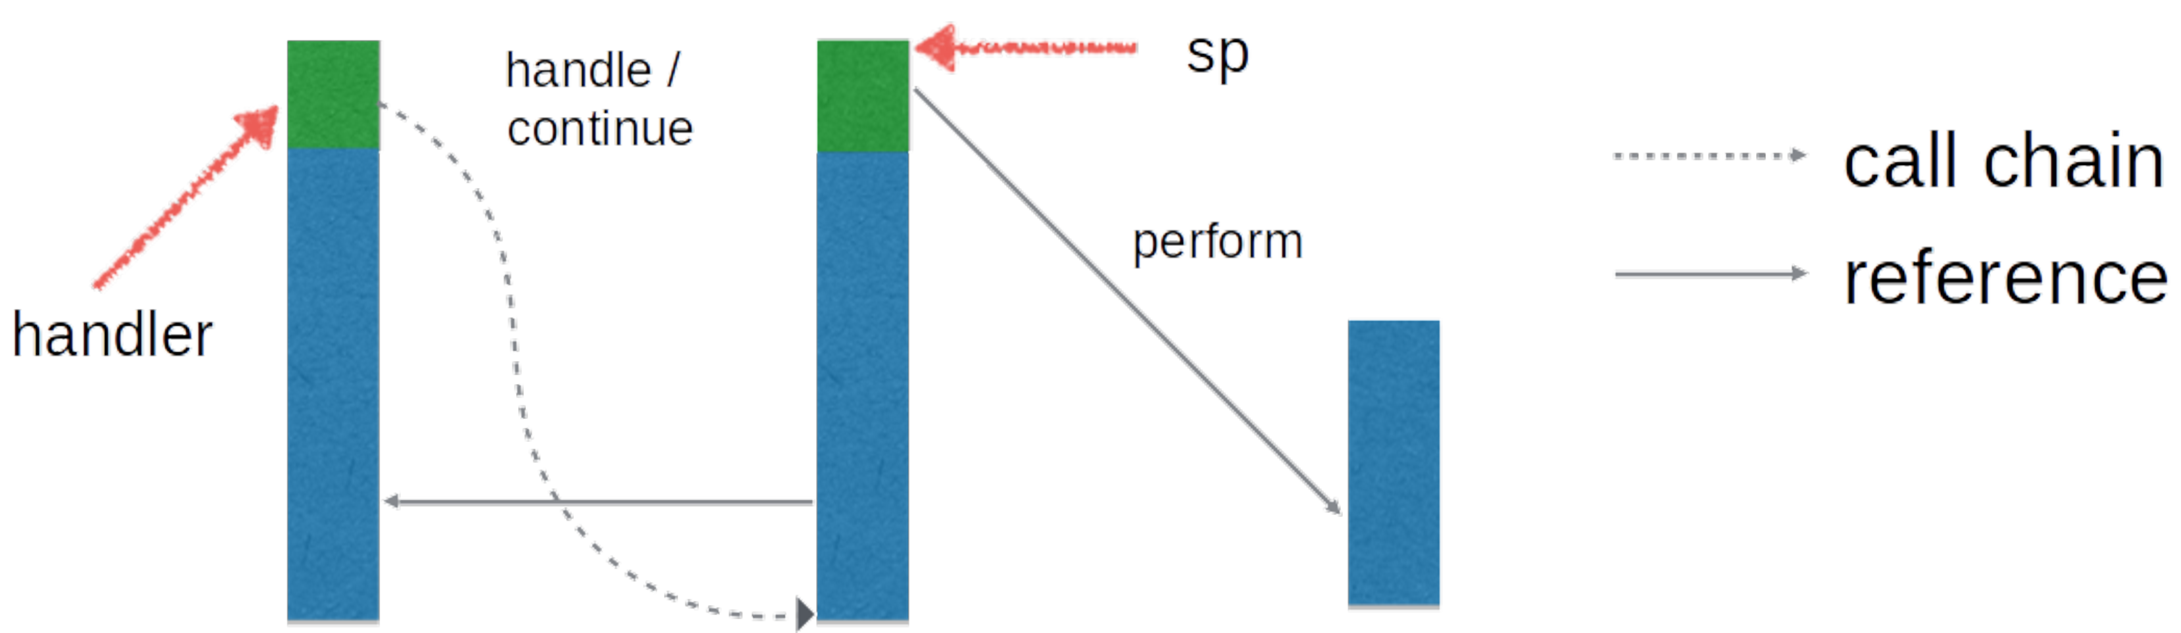
\includegraphics[width = 0.9\textwidth]{./imp3}
\end{center}
\end{frame}

\begin{frame}
\frametitle{Fibers}
\begin{itemize}
\setlength\itemsep{2em}
\item Stack overflow checks for OCaml functions
\item Simple static analysis eliminates many checks
\item FFI calls are more expensive due to stack switching
\end{itemize}
\end{frame}

\begin{frame}[fragile]
\frametitle{Fibers}
\begin{center}
Normalized time (lower is better) \\[2em]
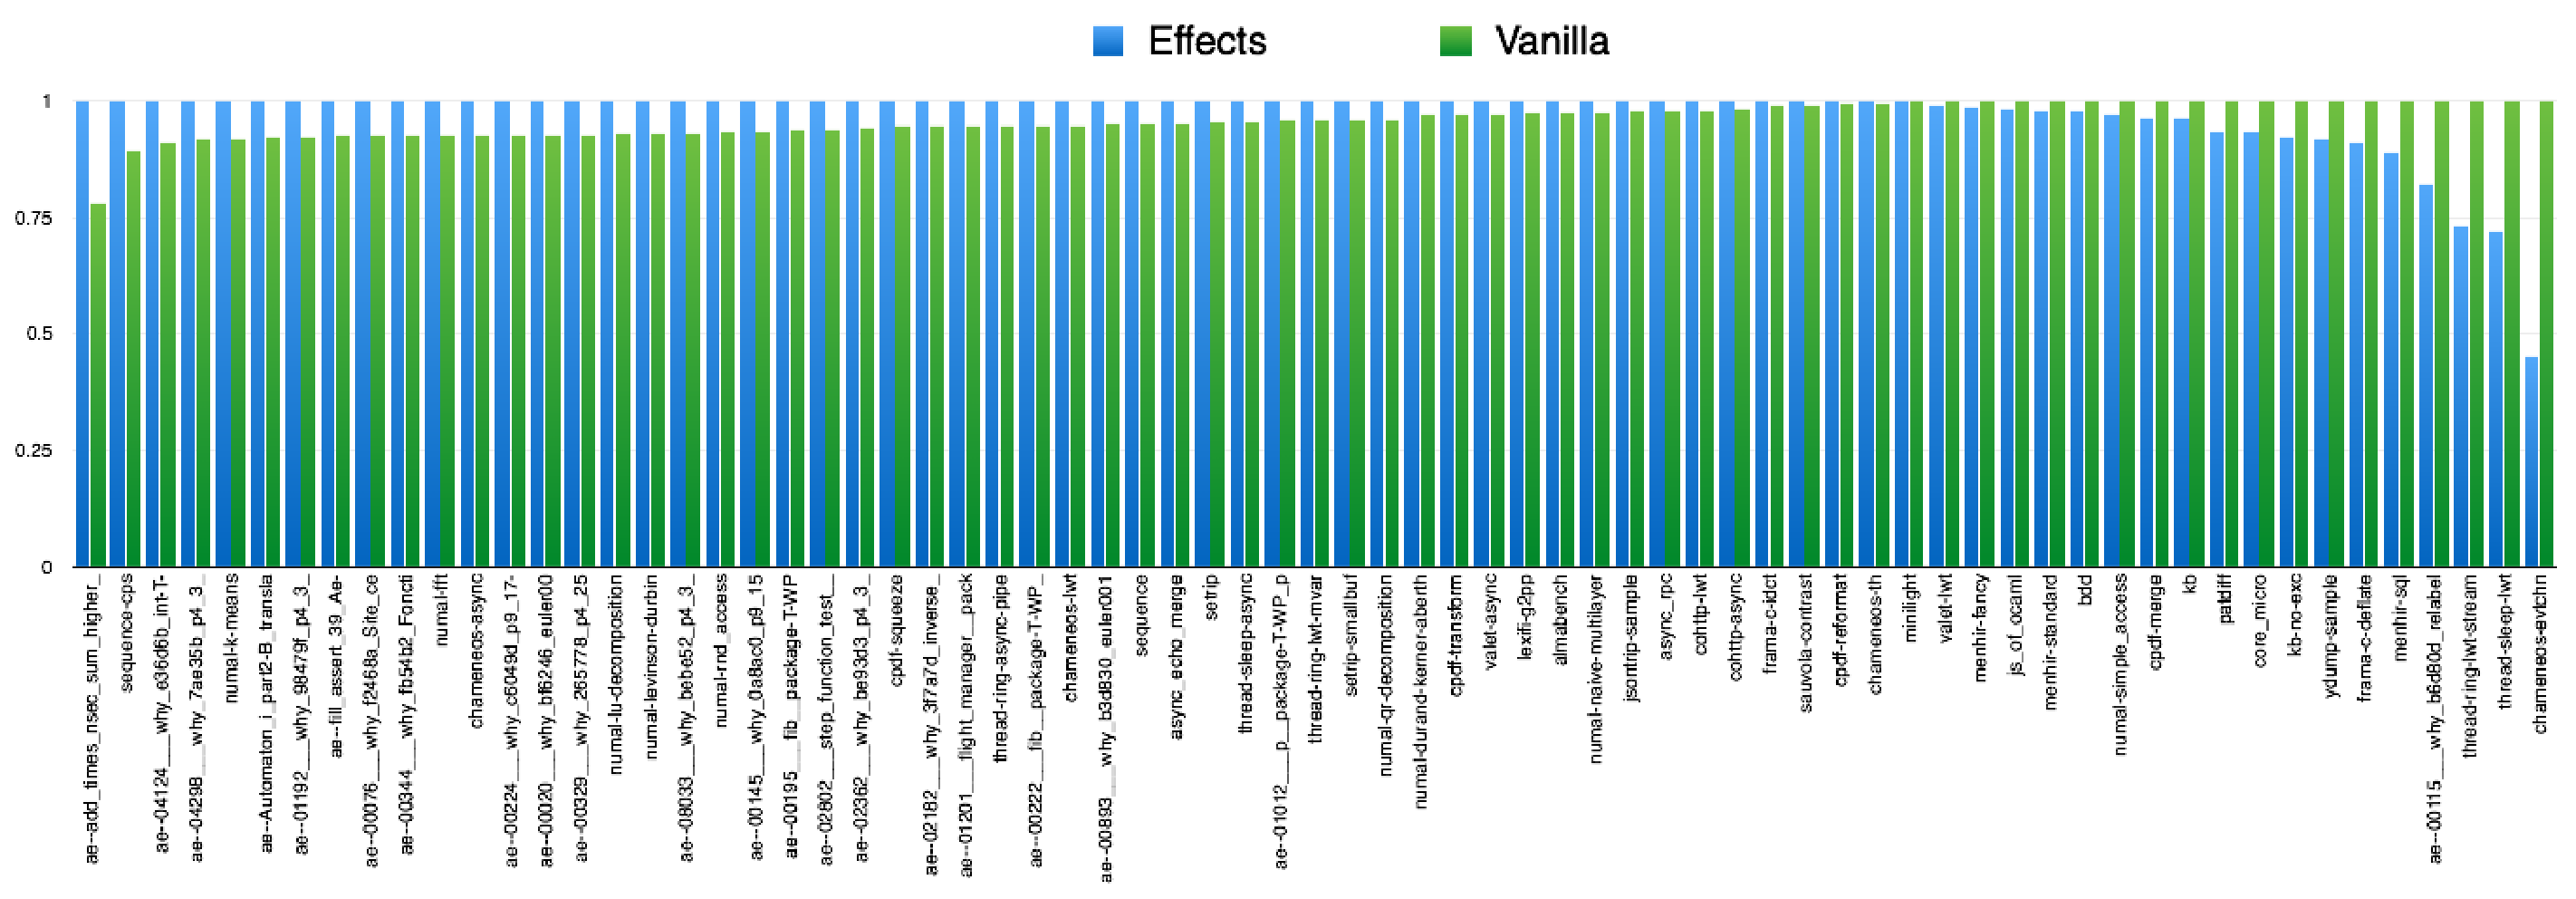
\includegraphics[width = 0.9\textwidth]{./fibers} \\[2em]
Fibers around 0.9\% slower
\end{center}
\end{frame}

\begin{frame}[c]
\begin{center}
\Huge Algebraic effects for concurrency
\end{center}
\end{frame}

\begin{frame}[fragile]
\frametitle{Concurrency effects}
\begin{lstlisting}[style=ocaml]
effect Async : ('a -> 'b) * 'a -> 'b promise
effect Await : 'a promise -> 'a

effect Write :
  file_descr * bytes * int * int -> int
with function Write(fd, buf, ofs, len) ->
  Unix.write fd buf ofs len
(**$\ldots$*)
\end{lstlisting}
\end{frame}

\begin{frame}[fragile]
\frametitle{Scheduler}
\begin{lstlisting}[style=ocaml]
let rec schedule state =
  if Queue.is_empty state.run_q then
    if empty state.reads &&
       empty state.writes then ()
    else select state
  else
    Queue.pop state.run_q ()
\end{lstlisting}
\end{frame}

\begin{frame}[fragile]
\frametitle{Scheduler}
\begin{lstlisting}[style=ocaml]
let wait state p k =
  match !p with
  | Done v -> continue k v
  | Waiting l ->
      p := Waiting (k::l);
      schedule state

let finish state p v =
  match !p with
  | Waiting l ->
      p := Done v;
      List.iter (fun k ->
        Queue.push (fun () -> continue k v)
          state.run_q)
        l
  | _ -> assert false
\end{lstlisting}
\end{frame}

\begin{frame}[fragile]
\frametitle{Scheduler}
\begin{lstlisting}[style=ocaml]
let rec run state p f x ->
  match f x with
  | v -> finish state p v; schedule state
  | effect Async(f, x), k ->
     let p = promise () in
     Queue.push (fun () -> continue k p)
       state.run_q;
     run state p f x
  | effect Await p, k -> wait state p k
\end{lstlisting}
\end{frame}

\begin{frame}[fragile]
\frametitle{Interface}
\begin{lstlisting}[style=ocaml]
val async : ('a -> 'b) -> 'a -> 'b future
val await : 'a future -> 'a

val write :
  file_descr -> bytes -> int -> int -> int
(**$\ldots$*)

val run : (unit -> unit) -> unit
\end{lstlisting}
\end{frame}

\begin{frame}[c]
\begin{center}
\Huge An effect system for OCaml
\end{center}
\end{frame}

\begin{frame}[fragile]
\frametitle{Effect system}
\begin{lstlisting}[style=ocamlgrammar]
A,B,... DEF ETC       BAR A $\RowTo$ B
\end{lstlisting}
\begin{prooftree}
\AxiomC{$\Context \Et \Var{x} \HasType \Var{A} \VDash \Var{e}
         \HasType \Var{B} \HasEffect \Var{\Row}$}
\alwaysSingleLine
\UnaryInfC{$\Context \VDash \lambda \Var{x} . \Var{e}
            \HasType \Var{A} \RowTo \Var{B} \HasEffect \Text{[]}$}
\end{prooftree}
\begin{prooftree}
\AxiomC{$\Context \VDash \Var{e}
         \HasType \Var{A} \RowTo \Var{B}
         \HasEffect \Var{\Row} $}
\AxiomC{$\Context \VDash \Var{e^\prime}
         \HasType \Var{A} \HasEffect \Var{\Row}$}
\alwaysSingleLine
\BinaryInfC{$\Context \VDash \Var{e} \; \Var{e^\prime}
             \HasType \Var{B} \HasEffect \Var{\Row}$}
\end{prooftree}
\end{frame}

\begin{frame}
\frametitle{Requirements}
\begin{block}{Soundness}
  If a program receives a type $A \HasEffect \Row$, every potential effect
  \texttt{e} should be captured in $\Row$.
\end{block}
\begin{block}{Usefulness}
  An effect system that annotates each program with every possible
  effect there is, is obviously sound, but not very useful. Thus, an
  effect information should not mention an effect that is guaranteed not
  to happen.
\end{block}
\begin{block}{Backwards compatibility}
  We want each program that was typable before introducing effects to
  remain typable.
\end{block}
\end{frame}

\begin{frame}[fragile]
\frametitle{Requirements}
\begin{lstlisting}[style=ocaml]
if (**$e$*) then perform (**$E_1$*)
else perform (**$E_2$*)
\end{lstlisting}
\begin{block}{}<2->
Two established approaches to providing the required flexibility:
\begin{itemize}
\item Subtyping
\item Row polymorphism
\end{itemize}
\end{block}
\end{frame}

\begin{frame}
\frametitle{Subtyping}
\begin{prooftree}
\AxiomC{$\Context \VDash \Var{e} \HasType \Var{A} \HasEffect \Var{\Row}$}
\AxiomC{$\Subtype{\Var{A}}{\Var{B}}$}
\alwaysSingleLine
\BinaryInfC{$\Context \VDash \Var{e} \HasType \Var{B} \HasEffect \Var{\Row}$}
\end{prooftree}
Full implicit subtyping is difficult to add to OCaml:
\begin{itemize}
\item OCaml supports invariant type parameters.
\item Requires \emph{constrained types} of the form
  $A | \mathcal{C}$ where $\mathcal{C}$ is a set of constraints between
  type parameters.
\item Constrained types do not interact well with OCaml's module system.
\item Constraint generation needs to be directed to correctly track
  variance.
\end{itemize}
\end{frame}

\begin{frame}[fragile]
\frametitle{Row polymorphism}
\begin{lstlisting}[style=ocamlgrammar]
ROW DEF [ EFF    $\Or$ ROW  ] BAR [ $\Rvar$ ] BAR [ ]
\end{lstlisting}
\begin{prooftree}
\AxiomC{$\Equal{\Row}{\Row^\prime}$}
\alwaysSingleLine
\UnaryInfC{$\Equal{[\Eff \Or \Row]}{[\Eff \Or \Row^\prime]}$}
\end{prooftree}
\begin{equation*}
\Equal{[\Eff \Or \Eff^\prime \Or \Row]}
      {[\Eff^\prime \Or \Eff \Or \Row]}
\end{equation*}
\end{frame}

\begin{frame}
\frametitle{Row polymorphism}
\begin{prooftree}
\AxiomC{$\Var{E} \HasType \Var{A} \to \Var{B} \in \Var{\Eff}$}
\AxiomC{$\Context \VDash \Var{e}
         \HasType \Var{A} \HasEffect [ \Var{\Eff} \Or \Var{\Row} ]$}
\alwaysSingleLine
\BinaryInfC{$\Context \VDash \Keyword{perform} \; \Var{E} \; \Var{e}
             \HasType \Var{B}
             \HasEffect [ \Var{\Eff} \Or \Var{\Row} ]$}
\end{prooftree}
\end{frame}

\begin{frame}[fragile]
\frametitle{Row polymorphism}
\begin{lstlisting}[style=ocaml]
let raise msg = perform Raise msg;;
\end{lstlisting}
\begin{lstlisting}[style=ocaml]
val raise : string -[exn | !p]-> unit
\end{lstlisting}
\end{frame}

\begin{frame}
\frametitle{Row polymorphism}
\begin{prooftree}
\alwaysNoLine
\AxiomC{$\Context \VDash \Var{e} \HasType \Var{A}
         \HasEffect [\Var{\Eff} \Or \Var{\Row}]$}
\UnaryInfC{$\Context \Et \Var{x} \HasType \Var{A} \VDash \Var{e^\prime}
            \HasType \Var{B} \HasEffect \Var{\Row}$}
\AxiomC{$\Eff = \big\{ E_i \HasType \Var{C_i} \to \Var{D_i} \big\}$}
\UnaryInfC{$\Context \Et \Var{x_i} \HasType \Var{C_i} \Et \Var{k_i} \HasType
            \Text{(} \Var{D_i} \Text{,} \Var{B} \Text{)} \,\Text{cont} \VDash
            \Var{e^{\prime\prime}_i} \HasType \Var{B} \HasEffect \Var{\Row}$}
\alwaysSingleLine
\BinaryInfC{$\Context \VDash
            \begin{aligned}
           & \Keyword{match} \; \Var{e} \; \Keyword{with} \\
           & \Text{|} \; \Var{x} \; \Text{->} \; \Var{e^\prime} \\
           & \Text{|} \; \Keyword{effect} \; E_i \; \Var{x_i} \Text{,}
               \; \Var{k_i} \; \Text{->} \; \Var{e^{\prime\prime}_i}
            \end{aligned}
            \HasType \Var{B} \HasEffect \Var{\Row}$}
\end{prooftree}
\end{frame}

\begin{frame}[fragile]
\frametitle{Row polymorphism}
\begin{lstlisting}[style=ocaml]
let run f =
  match f () with
  | ret -> Ok ret
  | effect Raise msg, k -> Error msg
\end{lstlisting}
\begin{lstlisting}[style=ocaml]
val run : (unit -[exn | !p]-> 'a)
            -[!p]-> ('a, string) result
\end{lstlisting}
\end{frame}

\begin{frame}[fragile]
\frametitle{Row polymorphism}
\begin{lstlisting}[style=ocaml]
val old_fun : int -> int
\end{lstlisting}
\begin{lstlisting}[style=ocaml]
let new_fun p =
  if p then old_fun 10
  else perform Get
\end{lstlisting}
{\color{red}
\begin{verbatim}
Error: This expression performs effect [state| !r], but
       it was expected to perform [].
\end{verbatim}}
\end{frame}

\begin{frame}[fragile]
\frametitle{Row polymorphism}
\begin{lstlisting}[style=ocaml]
type t = int -> int
\end{lstlisting}
{\color{red}
\begin{verbatim}
Error: Unbound type parameter !r.
\end{verbatim}}
\end{frame}

\begin{frame}
\frametitle{A compromise}
\begin{prooftree}
\AxiomC{$\Context \VDash \Var{e}
         \HasType \forall \Var{\overline{\alpha}} \Var{\overline{\Rvar}}.
         \Var{A} \HasEffect \Var{\Row}$}
\AxiomC{$open^+(\Var{A}) = \forall \Var{\overline{\Rvar^\prime}} . \Var{B}$}
\alwaysSingleLine
\BinaryInfC{$\Context \VDash \Var{e}
             \HasType \Var{B}[
             \Var{\overline{C}} / \Var{\overline{\alpha}},
             \Var{\overline{\Row^\prime}} / \Var{\overline{\Rvar}},
             \Var{\overline{\Row^{\prime\prime}}} / \Var{\overline{\Rvar^\prime}} ]
             \HasEffect \Var{\Row}$}
\end{prooftree}
\begin{align*}
&open^+([ \Eff_1 | \ldots | \Eff_n ]) =
  \forall \Rvar . [ \Eff_1 | \ldots | \Eff_n | \Rvar ] \\
&open^+(A \RowTo B) =
  open^-(A) \xrightarrow{open^+{\Row}} open^+(B) \\
&\ldots
\end{align*}
\begin{align*}
&open^-([ \Eff_1 | \ldots | \Eff_n ]) =
  [ \Eff_1 | \ldots | \Eff_n ] \\
&open^-(A \RowTo B) =
  open^+(A) \xrightarrow{open^-{\Row}} open^-(B) \\
&\ldots
\end{align*}
\end{frame}

\begin{frame}[fragile]
\frametitle{A compromise}
\begin{lstlisting}[style=ocaml]
val old_fun : int -> int
\end{lstlisting}
\begin{lstlisting}[style=ocaml]
let new_fun p =
  if p then old_fun 10
  else perform Get
\end{lstlisting}
\begin{lstlisting}[style=ocaml]
val new_fun : bool -[state | !p]-> int
\end{lstlisting}
\end{frame}

\begin{frame}
\frametitle{A compromise}
\begin{prooftree}
\AxiomC{$\Context \VDash \Var{e} \HasType \Var{A} \HasEffect []$}
\AxiomC{$\Var{\overline{\alpha}} \Var{\overline{\Rvar}} \notin ftv(\Context)$}
\AxiomC{$close^+(
         \forall \Var{\overline{\alpha}} \Var{\overline{\Rvar}} .
         \Var{A}) =
         \forall \Var{\overline{\alpha}} \Var{\overline{\Rvar^\prime}} .
         \Var{B}$}
\alwaysSingleLine
\TrinaryInfC{$\Context \VDash \Var{e}
             \HasType \forall \Var{\overline{\alpha}} \Var{\overline{\Rvar^\prime}} .
             \Var{B}
             \HasEffect \Var{\Row}$}
\end{prooftree}
\begin{equation*}
close^+(\forall \overline{\alpha} \overline{\Rvar} .A) =
  \forall \overline{\alpha} \overline{\Rvar} .
    A[\overline{[]} / closable^+(A, \overline{\Rvar})]
\end{equation*}
\begin{align*}
&closable^+(\Row, \overline{\Rvar}) = \overline{\Rvar} \\
&closable^+(A \RowTo B, \overline{\Rvar}) =
  closable^-(A, \overline{\Rvar})
  \cap closable^+{\Row}
  \cap closable^+(B) \\
&\ldots
\end{align*}
\begin{align*}
&closable^-([ \Eff_1 | \ldots | \Eff_n | \Rvar ], \overline{\Rvar}) =
  \overline{\Rvar} \setminus \Rvar \\
&closable^-(A \RowTo B, \overline{\Rvar}) =
  closable^+(A, \overline{\Rvar})
  \cap closable^-(\Row)
  \cap closable^-(B) \\
&\ldots
\end{align*}
\end{frame}

\begin{frame}[fragile]
\frametitle{A compromise}
\begin{lstlisting}[style=ocaml]
let raise msg = perform Raise msg;;
\end{lstlisting}
\begin{lstlisting}[style=ocaml]
val raise : unit -[exn]-> int
\end{lstlisting}
\end{frame}

\begin{frame}[fragile]
\frametitle{Defining effects}
\begin{lstlisting}[style=ocaml]
effect state =
  | Get : int
  | Put : int -> unit
\end{lstlisting}
\end{frame}

\begin{frame}[fragile]
\frametitle{Defining effects}
\begin{lstlisting}[style=ocaml]
effect fail =
  | Failure of string
\end{lstlisting}
\end{frame}

\begin{frame}[fragile]
\frametitle{Purity}
Define a built-in abstract effect:
\begin{lstlisting}[style=ocaml]
effect io
\end{lstlisting}
Treat OCaml's built-in side-effects as performing it:
\begin{lstlisting}[style=ocaml]
val ref : 'a -[io]-> 'a ref
\end{lstlisting}
As with Haskell, divergence and raising exceptions are still considered
``pure''.
\end{frame}

\begin{frame}[c]
\begin{center}
\Huge Usability
\end{center}
\end{frame}

\begin{frame}[fragile]
\frametitle{Useful short-hands}
\begin{lstlisting}[style=ocaml]
->    =    -[io]->

->>   =    -[]->

(**$\sim$*)>    =    -[io | !(**$\sim$*)]->

(**$\sim$*)>>   =    -[!(**$\sim$*)]->
\end{lstlisting}
\end{frame}

\begin{frame}[fragile]
\frametitle{Useful short-hands}
\begin{lstlisting}[style=ocaml]
val map : ('a (**$\sim$*)>> 'b) ->> 'a list (**$\sim$*)>> 'b list
\end{lstlisting}
\begin{lstlisting}[style=ocaml]
val map : ('a (**$\sim$*)> 'b) ->> 'a array (**$\sim$*)> 'b array
\end{lstlisting}
\end{frame}

\begin{frame}[fragile]
\frametitle{Updating the standard library}
\begin{itemize}
\item The standard library is 101 files totalling 23675 lines
\item
\begin{verbatim}
72 files changed, 3 insertions(+),
160 deletions(-), 4618 modifications(!)
\end{verbatim}
\item 2410 lines: changing value specifications -- no explict effect
  variables needed
\begin{lstlisting}[style=ocaml]
-val map : ('a -> 'b) -> 'a list -> 'b list
+val map : ('a (**$\sim$*)>> 'b) ->>
             'a list (**$\sim$*)>> 'b list
\end{lstlisting}
\item 220 lines: avoiding polymorphic comparison
\begin{lstlisting}[style=ocaml]
-if x = y then
+if Int_compare.(x = y) then
\end{lstlisting}
\end{itemize}
\end{frame}

\begin{frame}[fragile]
\frametitle{Updating the standard library}
\begin{itemize}
\item 214 lines: pure versions of Set and Map -- implementations shared
  with impure versions but some boilerplate required
\begin{lstlisting}[style=ocaml]
+module type OrderedTypePure =
+  sig
+    type t
+    val compare: t ->> t ->> int
+end
\end{lstlisting}
\item 1892 lines: Adding an effect parameter to format strings.
\begin{lstlisting}[style=ocaml]
-val printf :
  ('a, out_channel, unit) format -> 'a
+val printf :
  ('a, out_channel, unit, ![io | !p]) format
    -[io | !p]-> 'a
\end{lstlisting}
\end{itemize}
\end{frame}

\begin{frame}[fragile]
\frametitle{Updating the standard library}
\begin{itemize}
\item And 2 type annotations:
\begin{lstlisting}[style=ocaml]
-let printers = ref []
+let printers :
    (exn -> string option) list ref =
      ref []

-let locfmt = format_of_string "...";;
+let locfmt : _ format6e = "...";;
\end{lstlisting}
\end{itemize}
\end{frame}

\begin{frame}[fragile]
\frametitle{Replacing \texttt{Not\_found} the standard library}
\begin{itemize}
\item
\begin{verbatim}
34 files changed, 31 insertions(+),
332 modifications(!)
\end{verbatim}
\item 130 lines changing \lstinline[style=ocaml]{raise} to
  \lstinline[style=ocaml]{perform} and \lstinline[style=ocaml]{with} to
  \lstinline[style=ocaml]{with effect}
\begin{lstlisting}[style=ocaml]
-raise Not_found
+perform Not_found
\end{lstlisting}
\item 158 lines: updating value specifications
\begin{lstlisting}[style=ocaml]
-val find :
   ('a (**$\sim$*)>> bool) ->> 'a list (**$\sim$*)>> 'a
+val find :
   ('a -[not_found | !p]-> bool) ->>
      'a list -[not_found | !p]-> 'a
\end{lstlisting}
\end{itemize}
\end{frame}

\begin{frame}[fragile]
\frametitle{Replacing \texttt{Not\_found} in the standard library}
\begin{itemize}
\item 35 lines: adding handlers for cases that were not expected to occur
\begin{lstlisting}[style=ocaml]
+try
   min_binding t
+with effect Not_found -> assert false
\end{lstlisting}
\item 1 type annotation
\begin{lstlisting}[style=ocaml]
-and parse_integer str_ind end_ind =
+and parse_integer :
   int ->> int -> int * int =
\end{lstlisting}
\end{itemize}
\end{frame}

\begin{frame}[fragile]
\frametitle{Replacing \texttt{Not\_found} in the standard library}
\begin{itemize}
\item 2 coercions related to sharing implementations between the pure
  and impure versions of Set/Map
\begin{lstlisting}[style=ocaml]
+let compare_not_found =
+ (Ord.compare
+   : _ -[.. as ![] E.eff]-> _
+       -[.. as ![] E.eff]-> _
+  :> _ -[not_found | .. as ![] E.eff]-> _
+       -[not_found | .. as ![] E.eff]-> _)
\end{lstlisting}
\end{itemize}
\end{frame}

\begin{frame}[fragile]
\frametitle{Typed concurrency effects}
\begin{lstlisting}[style=ocaml]
effect async =
  | Async :
      ('a -[aio|async|io]-> 'b) * 'a ->
        'b promise
  | Await : 'a promise -> 'a

effect aio =
  | Write :
      file_descr * bytes * int * int -> int
  | (**$\ldots$*)
with function
  | Write(fd, buf, ofs, len) ->
      Unix.write fd buf ofs len
  | (**$\ldots$*)
\end{lstlisting}
\end{frame}

\begin{frame}[fragile]
\frametitle{Typed concurrency interface}
\begin{lstlisting}[style=ocaml]
effect async

val async :
  ('a -[async|aio|io]-> 'b) ->> 'a
    -[async]-> 'b promise
val await : 'a promise -[async]-> 'a

effect aio with function

val write :
  file_descr ->> bytes ->> int ->> int
    -[aio]-> int

val run : (unit -[async|aio|io]-> unit) -> unit
\end{lstlisting}
\end{frame}

\begin{frame}[c]
\begin{center}
\Huge Challenges
\end{center}
\end{frame}

\begin{frame}[fragile]
\frametitle{Affine continuations and purity}
\begin{lstlisting}[style=ocaml]
effect yield = Yield : unit

let f () =
  match perform Yield with
  | _ -> `None
  | effect Yield, k -> `Some k

let x = f ()
let y = f ()

let _ =
  match x, y with
  | `Some x, `Some y ->
      continue x (), continue y ()
  | p -> p
\end{lstlisting}
\end{frame}

\begin{frame}[fragile]
\frametitle{Affine continuations and purity}
\begin{lstlisting}[style=ocaml]
effect yield = Yield : unit

let f () =
  match perform Yield with
  | _ -> `None
  | effect Yield, k -> `Some k

let x = f ()
let y = x

let _ =
  match x, y with
  | `Some x, `Some y ->
      continue x (), continue y ()
  | p -> p
\end{lstlisting}
\end{frame}

\begin{frame}[fragile]
\frametitle{Effect parameters and abstraction}
\begin{lstlisting}[style=ocaml]
effect 'a state =
    | Get : 'a
    | Put : 'a -> unit

let fold f l init =
  let comp =
    match
       List.iter
         (fun x ->
            perform Put (f x (perform Get))) l
    with
    | () -> fun s -> s
    | effect Get, k -> fun s -> continue k s s
    | effect Put s, k ->
        fun _ -> continue k () s
  in
  comp init
\end{lstlisting}
\end{frame}

\begin{frame}[fragile]
\frametitle{Effect parameters and abstraction}
\begin{lstlisting}[style=ocaml]
let fold (type acc) f l init =
  let effect state =
    | Get : acc
    | Put : acc -> unit in
  let comp =
    match
       List.iter
         (fun x ->
            perform Put (f x (perform Get)))
         l
    with
    | () -> fun s -> s
    | effect Get, k -> fun s -> continue k s s
    | effect Put s, k ->
        fun _ -> continue k () s
  in
  comp init
\end{lstlisting}
\end{frame}

\begin{frame}[fragile]
\frametitle{Effect parameters and abstraction}
\begin{lstlisting}[style=ocaml]
module M : sig
  effect 'a state2
  val pfrm : unit -[int state2]-> unit
  val handle : ('a -[int state2 | !p]-> 'b) ->
                 'a -[!p]-> 'b
end = struct
  effect 'a state2 = 'a state
  let pfrm () = perform Put 0
  let handle f x =
    match f x with
    | y -> y
    | effect Get, k = continue k 0
    | effect Put _, k = continue k ()
end
\end{lstlisting}
\end{frame}

\begin{frame}[fragile]
\frametitle{Effect parameters and abstraction}
\begin{lstlisting}[style=ocaml]
let _ =
  M.handle (fun () ->
    let comp =
      match M.pfrm (); perform Get with
      | x -> fun _ -> x
      | effect Get, k ->
          fun s -> continue k s s
      | effect Put s, k ->
          fun _ -> continue k () s
    in
    print_string (comp "init"))
\end{lstlisting}
\end{frame}

\begin{frame}[fragile]
\frametitle{Nominative vs Structural}
\begin{itemize}
\item Nominative definitions in OCaml are all abstractable. Can't really
  restrict abstraction whilst effects are treated nominatively.
\item Could avoid abstraction by treating effects structurally:
\begin{lstlisting}[style=ocaml]
let get : unit -[ `Get : 'a ]-> 'a =
  fun () -> perform `Get
\end{lstlisting}
\item Allows parameterised effects
\item How to handle \lstinline[style=ocaml]{io} (which is an abstract effect)?
\item How to handle default handlers?
\end{itemize}
\end{frame}

\begin{frame}
\frametitle{So...}
\begin{itemize}
\item Algebraic effects and handlers are a good mechanism for modelling
  effects
\item Algebraic effects and handlers enable users to efficiently
  and composably implement their own concurrent schedulers
\item Effect systems can be used to manage algebraic effects as well as
  side-effects more generally
\item It is possible to create effect systems that are both usable and
  backwards compatible with existing languages like OCaml
\end{itemize}
\end{frame}

\end{document}
